\RequirePackage{iftex}
\ifXeTeX\PassOptionsToPackage{xetex}{hyperref}\fi
\documentclass{lmcs}
\usepackage[T1]{fontenc}
\usepackage{amsmath,amsfonts,amssymb,mathtools}
\usepackage{booktabs,array,graphicx,needspace}
\newcommand{\Ftwo}{\mathbb{F}_2}
\newcommand{\Var}{\mathsf{Var}}
\newcommand{\Chk}{\mathsf{Chk}}
\newcommand{\Nb}{\mathcal{N}}
\newcommand{\xor}{\oplus}
\newcommand{\bigxor}{\bigoplus}
\newcommand{\starE}{\star}
\newcommand{\Edges}{\mathcal{E}}
\newtheorem*{adequacyprinciple}{Proposition (abstract adequacy principle)}
\newcommand{\RepoURL}{\url{https://github.com/cero1979/SELLTC}}
\keywords{LDPC codes, binary erasure channel, certifying algorithms,
subexponential linear logic, multiset rewriting, trace adequacy, Lean}
% The current class's empty first-page header exceeds its fixed boxes under
% Tectonic. Enlarge only those header boxes; keep headheight+headsep unchanged
% so the text block and its margins retain the LMCS geometry.
\makeatletter
\patchcmd{\ps@firstpage}{30 pt}{36 pt}{}{\PackageError{SELLTC}{Header patch failed}{}}
\patchcmd{\ps@firstpage}{30 pt}{36 pt}{}{\PackageError{SELLTC}{Header patch failed}{}}
\patchcmd{\ps@firstpage}{30 pt}{36 pt}{}{\PackageError{SELLTC}{Header patch failed}{}}
\dimen@=\headheight
\advance\dimen@ by -40pt
\advance\headsep by \dimen@
\headheight=40pt
\makeatother
\begin{document}
\title[Exact Trace Adequacy for LDPC Peeling]{Exact Trace Adequacy for LDPC Peeling:\texorpdfstring{\\}{ }Delayed Propagation and Residual Certificates}
\author[C.~Ram\'irez~Ovalle]{Carlos Ram\'irez Ovalle\lmcsorcid{0000-0002-4254-5610}}
\address{Pontificia Universidad Javeriana, Cali, Colombia}
\email{carlosovalle@javerianacali.edu.co}
\begin{abstract}
Certifying hybrid LDPC decoding over the binary erasure channel requires
connecting local peeling steps with a residual algebraic result. In an
asynchronous specification, a solved variable may await propagation to
some checks while other solves proceed, so stored residuals need not
match the operational state. We give a pending-incidence invariant that
accounts for this delay. Our principal theorem establishes exact
trace adequacy: every rewrite execution, with arbitrary interleaving of
solving and propagation, emits the same valid operational trace under
projection; every prescribed valid trace has a rewrite realization with
its exact logged endpoint after propagation normalization. Empty and
partial traces are included. An abstract proposition isolates the
simulation, canonical normalization and local lifting hypotheses behind
this correspondence. Residual linear algebra then supplies independently
checkable compatible-completion or left-kernel infeasibility certificates.
Trace replay certifies a local operational explanation in addition to
the final-word predicate already established by direct checking.
A Lean development mechanizes the canonical LDPC correspondence and
certificate results within stated boundaries; finite tests and retained
experiments assess an independent Python implementation and its checking
costs. The subexponential presentation exposes the resource discipline,
while an event-preserving translation shows that its two persistent
labels are inessential for these operational rules.
\end{abstract}
\maketitle

\section{Introduction}
Hybrid decoding over the binary erasure channel (BEC) combines local
peeling with a linear solve on the remaining erasures. An untrusted
producer can accompany its result with a certificate checked independently
of that producer. The central question here is how an asynchronous,
resource-sensitive account of peeling can certify exactly the declared
sequence of local assignments when propagation is delayed. Our principal
result, Theorem~\ref{thm:sem-adequacy}, relates these rewrite executions
to the same operational peeling traces in both directions and identifies
their exact logged endpoints after normalization.

Four levels organize the construction. At the \emph{algorithmic level},
classical peeling forces erased variables and Gaussian elimination solves
the residual system
\cite{RichardsonUrbanke2008,BurshteinMiller2004ML}. At the
\emph{certificate level}, witnesses separate the producer from trusted
checking, following certifying algorithms
\cite{McConnellEtAl2011,AlkassarEtAl2013,Necula1997PCC}. Here a successful
witness completes the residual equations, while a left-kernel witness
certifies inconsistency. These two levels provide the decoding problem
and its algebraic contract.

The \emph{asynchronous semantic level} explains each declared peeling
assignment. Once a variable has been solved, some neighboring checks may
still await its value while another Solve event occurs elsewhere.
Consequently a stored degree can exceed the number of genuinely unknown
neighbors, and a stored syndrome can omit known values. Treating such a
context as fully updated would invalidate the simulation argument.
Moreover, the final multiset contains persistent log atoms; their exact
presence must be retained in a reachability theorem, even though their
multiset alone cannot recover chronological order.

The invariant makes these two issues explicit. Write $K$ for the current
partial assignment, $Q_j$ for the incidences still pending at check $j$,
and $p_j$ for its stored syndrome. Pending incidences include every unknown
neighbor and may also include delayed known neighbors
$D_j=Q_j\cap\operatorname{dom}K$. If $d(j)$ and $s(j)$ are the actual
operational degree and syndrome, then
\[
 |Q_j|=d(j)+|D_j|,\qquad
 s(j)=p_j\xor\bigxor_{i\in D_j}K(i).
\]
Propagation removes a known pending incidence while leaving the
operational projection unchanged. A Solve event is justified at its
forcing check even if other checks still have delayed incidences.
Propagation terminates with a unique normal form, where the stored and
operational residuals agree. These facts make the arbitrary-interleaving
soundness direction of Theorem~\ref{thm:sem-adequacy} possible. Its converse
uses local enablement in normalized contexts to realize each prescribed
operational trace, retaining the accumulated log exactly.

The \emph{logical presentation level} exposes reusable information and
consumable residual resources through a vocabulary inspired by
subexponential linear logic (SELL). Static facts and learned values occupy
two persistent zones. Proposition~\ref{prop:sem-label-erasure} identifies
what this presentation contributes: the zones express an intended access
discipline, but their differentiated labels can be erased while preserving
the specified event-labelled transitions. The trace correspondence depends
on the asynchronous resource updates and their invariant. It does not
require an expressive advantage of two persistent labels or an adequacy
claim for a focused logical calculus.

The contributions are as follows.
\begin{enumerate}
\item \emph{Certificate algebra.} A residual-solution bijection gives
success soundness and left-kernel failure soundness and completeness for
every specified valid finite trace, including a partial or empty trace
(Section~\ref{sec:certificates}). It separates compatible completion,
uniqueness and exact recovery.
\item \emph{Invariant and normalization.} Exact token
multiplicities and pending-incidence equations support invariant
preservation, silent stuttering and a unique propagation normal form
(Section~\ref{sec:sem-invariant}). Only propagation is claimed confluent.
\item \emph{Exact trace adequacy.} Theorem~\ref{thm:sem-adequacy} proves
arbitrary-interleaving soundness and completeness for the very same
requested trace, with a logged normalized endpoint. A preceding abstract
proposition isolates the sufficient hypotheses, including the local
lifting needed for completeness (Section~\ref{sec:sem-adequacy}).
\item \emph{Formal and executable evidence.} A canonical Lean development
mechanizes the LDPC trace correspondence and scoped certificate results.
Independent Python checkers, finite differential tests and a reproducible
cost study provide separate implementation evidence
(Sections~\ref{sec:lean}--\ref{sec:results}).
\end{enumerate}

Direct verification of a proposed binary word already establishes
$Hx=0$ and agreement with all visible symbols. Trace replay certifies a
local operational explanation, not a stronger final-word correctness
predicate: every declared assignment must be forced by a degree-one check
in the preceding state. This is a property of the supplied explanation,
not an attestation of the producer's actual internal history. Both checks
have a linear sparse upper bound; the retained measurements show direct
checking to be faster, so the additional trace evidence has an explicit
measured cost.

The source repository is \RepoURL. The representation and implementation
boundaries are stated in Section~\ref{sec:lean}; Python is independently
implemented, not extracted from Lean. Current access restrictions and
release requirements are recorded in the companion readiness report;
this manuscript does not assert that a public archival release exists.

\section{Coding and operational preliminaries}
\label{sec:core}
Let $H\in\Ftwo^{m\times n}$, with variable set $\Var=\{1,\ldots,n\}$,
check set $\Chk=\{1,\ldots,m\}$, and Tanner edges
$\Edges=\{(j,i):H_{ji}=1\}$. Write $\Nb(j)=\{i:H_{ji}=1\}$ and
$C=\{x\in\Ftwo^n:Hx=0\}$. Vectors are columns throughout.
The matrix need not have full row rank, and empty rows, empty columns,
$m=0$ and $n=0$ are allowed. Sparsity is needed for the implementation
bounds, not for the algebraic theorems. LDPC decoding and its standard
iterative and algebraic ingredients are classical
\cite{Gallager1962,RichardsonUrbanke2008,LubyMitzenmacherShokrollahiSpielman2001,BurshteinMiller2004ML}.

A received word is $y\in\{0,1,\starE\}^n$. A partial assignment
$K:\Var\rightharpoonup\Ftwo$ has unknown set
$U=\Var\setminus\operatorname{dom}K$. A full word $x$ extends $K$ if
$x_i=K(i)$ whenever $K(i)$ is defined. Initially $K_0(i)=y_i$ at each
nonerased coordinate. For an assignment $K$, define
\begin{equation}\label{eq:operational-state}
 s_K(j)=\sum_{i\in\Nb(j)\cap\operatorname{dom}K}K(i),
 \qquad d_K(j)=|\Nb(j)\cap U|.
\end{equation}
All sums and matrix products are in $\Ftwo$, unless explicitly stated
otherwise. Thus addition is XOR. A coherent operational state
$\sigma=(K,U,s,d)$ has $s=s_K$ and $d=d_K$.

\begin{defi}[Operational peeling and trace]\label{def:peeling}
A triple $a=(j,i,b)$ is valid at $\sigma$ if
$\Nb(j)\cap U=\{i\}$ and $b=s(j)$. Its successor extends $K$ by
$K(i)=b$, removes $i$ from $U$, and, for every $\ell$ adjacent to $i$,
sets $s(\ell)\leftarrow s(\ell)+b$ and
$d(\ell)\leftarrow d(\ell)-1$. Other entries remain unchanged.
A trace $T=(a_1,\ldots,a_t)$ is valid from $y$ when every triple is valid
at the preceding state, starting at $K_0$. Traces may be empty or stop
before peeling is maximal. Every valid trace has $t\leq n$ because it
resolves a different unknown coordinate at every step.
\end{defi}

\begin{lem}[State meaning and preservation of completions]\label{lem:core-invariant}
Every state reached by a valid trace satisfies
\eqref{eq:operational-state}. Furthermore, every $x\in C$ agreeing with
the visible coordinates of $y$ extends its reached assignment $K$.
\end{lem}
\begin{proof}
Both state identities hold initially by definition. In a valid step,
$i$ was unknown, so adding it to $\operatorname{dom}K$ adds exactly $b$
to the known sum at each adjacent check and removes exactly one term
from the corresponding unknown-neighbor count. Nonadjacent checks
are unaffected. This proves the identities inductively.

Initially the assertion about $x$ is its assumed agreement with $y$.
Suppose $x$ extends the current $K$, and the next step is $(j,i,b)$.
Every neighbor of $j$ except $i$ is already known. Since the $j$-th
parity of $x$ is zero,
\[
 x_i=\sum_{h\in\Nb(j)\setminus\{i\}}x_h
     =\sum_{h\in\Nb(j)\cap\operatorname{dom}K}K(h)=s(j)=b.
\]
Thus $x$ extends the enlarged assignment too. Induction proves the
claim for the entire trace, including inputs that have no completion
(for which the assertion is vacuous).
\end{proof}

A nonempty $S\subseteq\Var$ is a \emph{stopping set} when every check
has either zero or at least two neighbors in $S$ \cite{DiEtAl2002Stopping}.
\begin{prop}[Stopping sets]\label{prop:core-stopping}
A maximal peeling run leaves a nonempty unknown set precisely when that
remaining set is a stopping set. Peeling removes all initial erasures
if and only if the initial erasure set contains no stopping set.
Here ``removes'' is a structural statement, not acceptance of a codeword.
\end{prop}
\begin{proof}
A step exists exactly when some check has one unknown neighbor.
Consequently a nonempty residual has no possible step exactly when it
is a stopping set. Now let $S$ be a stopping subset of the initial
unknown set. If peeling removed a member of $S$, consider the first
such removal. At its witnessing check all members of $S$ are still
unknown; that check touches $S$ and hence has at least two unknown
neighbors, contradicting degree one. Thus $S$ survives every run.
Conversely, a nonempty residual of a maximal run is itself a stopping
subset of the initial erasure set, by the first part. These implications
establish the characterization independently of the choice of eligible
checks. A degree-zero row with syndrome one may still rule out any
completion; it does not change the structural argument.
\end{proof}

\section{Residual algebra and certificate checking}\label{sec:certificates}
For the final unknown set $U$ of a valid trace, order its coordinates
in increasing order, let $H_U$ be the corresponding column restriction
of $H$, and put $r=(s(j))_{j\in\Chk}$. A residual assignment
$\rho\in\Ftwo^{|U|}$ fills those coordinates, and $K\cup\rho$ denotes
the resulting full word.

\begin{lem}[Residual equivalence]\label{lem:core-residual}
For a valid trace from $y$, the map $\rho\mapsto K\cup\rho$ is a
bijection between solutions of $H_U\rho=r$ and codewords agreeing with
all visible coordinates of $y$.
\end{lem}
\begin{proof}
For a word extending $K$, its $j$-th parity is
$s(j)+\sum_{i\in\Nb(j)\cap U}x_i$, by
Lemma~\ref{lem:core-invariant}. This parity is zero exactly when the
$j$-th equation of $H_Ux_U=r$ holds. Hence every residual solution
produces a compatible codeword. In the other direction,
Lemma~\ref{lem:core-invariant} says that every compatible codeword
extends $K$; its restriction to $U$ therefore solves the residual
system. Restriction and filling are inverse functions.
\end{proof}

\begin{defi}[Certificate formats and independent checker]\label{def:certificates}
A success certificate consists of the tag $\mathsf{success}$, a trace
$T$, and a binary witness $\rho$ of length $|U|$ after replay. A failure
certificate consists of the tag $\mathsf{failure}$, a trace $T$, and a
witness $\omega\in\Ftwo^m$.
The checker first rejects a trace longer than $n$ (or stops a streaming
trace after its $(n+1)$-st entry). It then validates the tag, triple
structure, integer index bounds, binary values and witness lengths. It initializes the coherent
state from $(H,y)$ and replays every triple according to
Definition~\ref{def:peeling}; it rejects at the first invalid step.
For success it accepts exactly when $H_U\rho=r$, returning $K\cup\rho$.
For failure it accepts exactly when
\begin{equation}\label{eq:separator}
 \omega^\top H_U=0,\qquad \omega^\top r=1.
\end{equation}
The checker uses only the supplied instance and certificate; it does
not invoke the decoder. All rows are checked, including zero-degree
rows. A schema-valid partial trace is allowed in both branches.
\end{defi}

A hybrid producer runs maximal peeling, constructs the residual, and
performs exact Gaussian elimination over $\Ftwo$. A solution produces
a success certificate; an inconsistent row produces a failure
certificate as described below. When $U$ is empty, the residual still
has $m$ equations: success requires $r=0$. Removing all erasures does
not justify skipping this check.

\begin{thm}[Success soundness]\label{thm:core-success}
If the checker accepts a success certificate and returns $x$, then
$x\in\Ftwo^n$, $Hx=0$, and $x_i=y_i$ at every nonerased coordinate.
\end{thm}
\begin{proof}
The validated binary witness and assignment $K$ define a binary word.
Replay only assigns initially unknown coordinates, so $K$ extends
$K_0$ and channel agreement holds. The accepted residual equation and
Lemma~\ref{lem:core-residual} establish $Hx=0$.
\end{proof}

\begin{lem}[Finite-field alternative]\label{lem:core-alternative}
For $A\in\Ftwo^{m\times q}$ and $r\in\Ftwo^m$, exactly one of the
following exists: a solution $z$ of $Az=r$, or a vector $\omega$ with
$\omega^\top A=0$ and $\omega^\top r=1$.
\end{lem}
\begin{proof}
They cannot both exist, since then
$1=\omega^\top r=\omega^\top Az=0$.
Suppose there is no solution. Let $W$ be the span of the columns of
$A$. Then $r\notin W$. Choose a basis of $W$; appending $r$ gives a
linearly independent family, which extends to a basis of the finite
space $\Ftwo^m$. Define a linear functional $f$ on this basis to be
zero on the basis of $W$, one on $r$, and zero on all additionally
chosen basis vectors. Unique basis expansion defines $f$ on the
whole space and proves its linearity. If $e_j$ are the coordinate
basis vectors and $\omega_j=f(e_j)$, then for every vector $v$,
$f(v)=\sum_j v_j f(e_j)=\omega^\top v$. Therefore $f$ annihilates
every column of $A$, while $f(r)=1$, giving the required witness.
The argument also covers $q=0$. If $m=0$, the zero vector of $\Ftwo^q$ is always
a solution and the inconsistent case cannot arise.
\end{proof}

\begin{prop}[Constructing a failure witness]\label{prop:core-extraction}
Suppose elementary row operations transform $[A\mid r]$ to
$[R\mid c]=M[A\mid r]$, where $M\in\Ftwo^{m\times m}$ records the
same operations on the identity matrix. If $R$ has a zero row $h$
with $c_h=1$, then $\omega^\top=e_h^\top M$ satisfies the failure
conditions. Row reduction of an inconsistent system always finds
such a row.
\end{prop}
\begin{proof}
Taking row $h$ of the displayed equality gives
$(e_h^\top M)A=R_{h,*}=0$ and $(e_h^\top M)r=c_h=1$.
Row swaps and adding one row to another are invertible over $\Ftwo$,
so they preserve solvability. In echelon form, if every zero coefficient
row has right-hand side zero, set all free variables to zero and solve
the pivot equations from bottom to top. This constructs a solution:
each pivot is one, later pivot variables are already assigned, and
zero rows impose no further condition. Consequently an inconsistent
echelon system must have a zero coefficient row with right-hand side
one. Redundant rows and zero-column matrices cause no exception.
\end{proof}

\begin{thm}[Failure soundness and certificate completeness]\label{thm:core-failure}
An accepted failure certificate excludes every codeword agreeing with
$y$. Conversely, for every $(H,y)$ and every valid finite trace $T$,
there is an accepted certificate of exactly one status: success if a
compatible codeword exists, and failure otherwise.
\end{thm}
\begin{proof}
For soundness, acceptance supplies \eqref{eq:separator}. By
Lemma~\ref{lem:core-residual}, any compatible codeword would supply
a residual solution. This contradicts Lemma~\ref{lem:core-alternative}.
For completeness, if a compatible codeword exists, its restriction
to $U$ supplies a success witness by the residual bijection.
Otherwise the residual is inconsistent and the finite-field
alternative supplies a failure witness. Both witnesses pass the
specified checks, and the two statuses cannot both be accepted by
the same alternative. This is an existence statement for a suitable
witness, not a claim that every alleged witness is accepted.
\end{proof}

\begin{prop}[Multiplicity and exact recovery]\label{prop:core-nullity}
If $H_U\rho=r$ is consistent and has rank $a$, it has exactly
$2^{|U|-a}$ solutions. Hence the compatible completion is unique if
and only if $|U|-a=0$. Under a clean erasure channel the transmitted
word is one of these completions; acceptance alone does not identify
it when more than one completion exists.
\end{prop}
\begin{proof}
For one solution $\rho_0$, every solution is uniquely of the form
$\rho_0+v$ with $v\in\ker H_U$, because
$H_U(\rho+\rho_0)=r+r=0$. Rank--nullity gives dimension $|U|-a$ for
this kernel. A basis of a $d$-dimensional binary vector space gives a
bijection with $\Ftwo^d$, which has $2^d$ elements. Apply the residual
bijection. On the clean channel the transmitted codeword agrees
with the visible symbols, proving the last assertion.
\end{proof}

\section{Likelihood, examples and trust boundary}\label{sec:interpretation}
For erasure probability $\epsilon\in[0,1]$, define the memoryless BEC
transition probability by
\[
 W_\epsilon(y\mid x)=\prod_{i=1}^n w_\epsilon(y_i\mid x_i),\qquad
 w_\epsilon(a\mid b)=
 \begin{cases}
  \epsilon,&a=\starE,\\
  1-\epsilon,&a=b,\\
  0,&a\in\Ftwo\text{ and }a\ne b.
 \end{cases}
\]
Maximum likelihood means maximizing this quantity over $x\in C$;
it does not impose a prior distribution on codewords.
\begin{prop}[BEC maximum likelihood]\label{prop:core-ml}
For every $\epsilon\in[0,1]$, a compatible codeword maximizes
$W_\epsilon(y\mid x)$ over $C$. If $0<\epsilon<1$ and a compatible
codeword exists, the maximizers are exactly the compatible codewords.
\end{prop}
\begin{proof}
Let $u$ and $k=n-u$ be the numbers of erased and visible coordinates.
Every compatible word has likelihood
$c=\epsilon^u(1-\epsilon)^k\geq0$; every incompatible word has a
zero factor and therefore likelihood zero. Thus no candidate has
likelihood greater than a compatible word. For interior $\epsilon$,
$c>0$, so the incompatible candidates are not maximizers. The product
definition handles the endpoints, with an empty product equal to one.
An observation impossible at an endpoint may give all candidates
likelihood zero; the first assertion still holds, but the second
need not. No posterior conditional on such a zero-probability event
is asserted.
\end{proof}

\begin{exa}[Peeling, stopping, ambiguity and impossibility]\label{exa:core}
All indices in these calculations are one-based; the software uses
zero-based indices.
\begin{enumerate}[label=(\alph*),leftmargin=*]
\item For
$H=\left(\begin{smallmatrix}1&1&0\\0&1&1\end{smallmatrix}\right)$ and
$y=(0,\starE,\starE)$, initially $s=(0,0)$ and $d=(1,2)$.
The step $(1,2,0)$ changes these to $s=(0,0)$, $d=(0,1)$.
The step $(2,3,0)$ leaves $U=\varnothing$ and $r=(0,0)$,
so the empty residual assignment certifies $x=(0,0,0)$.
\item For $H=(1\ 1)$ and $y=(\starE,\starE)$, the unknown set is
a stopping set and the empty trace is maximal. The residual equation
$\rho_1+\rho_2=0$ has solutions $(0,0)$ and $(1,1)$, rank one and
nullity one. Each is an ML completion, and neither is selected by
likelihood alone.
\item For
$H=\left(\begin{smallmatrix}1&1&0\\1&0&1\end{smallmatrix}\right)$,
$y=(\starE,0,1)$ and $T=\varnothing$, the residual is
$A=(1,1)^\top$, $r=(0,1)^\top$.
The witness $\omega=(1,1)^\top$ gives $\omega^\top A=0$ and
$\omega^\top r=1$. It certifies impossibility before any peeling.
Alternatively resolving $x_1=0$ from row one leaves no residual
variables and right-hand side $(0,1)$; $\omega=(0,1)^\top$ then
certifies the remaining degree-zero contradiction.
\item For $H=(1\ 1)$, a transmission of $(0,0)$ followed by one
visible flip and one erasure can yield $y=(1,\starE)$.
Peeling validly returns $(1,1)$, which passes both parity and channel
checks. The certificate is valid, but the transmitted word was not
recovered. Corruption need not make the observed constraints
inconsistent.
\end{enumerate}
\end{exa}

The trusted instance is the supplied pair $(H,y)$, including its
validated graph representation. The mathematical checker assumes
exact binary arithmetic; an executable deployment also trusts its
parser, checker implementation, interpreter/compiler and runtime.
The decoder and its residual solver need not be trusted. A Lean
proof of a mathematical function does not by itself verify an
independently written Python program or its execution environment.

An accepted trace certifies that the declared sequence is permitted
by the specification. It does not attest that an untrusted producer
actually followed this sequence internally. A valid partial trace,
or a permutation of independent steps that remains valid, must be
accepted. Malformed certificates, incompatible words and invalid
steps must be rejected. Rejection of a malformed failure witness
alone does not establish that a completion exists.

If the supplied matrix is corrupted, acceptance proves only the
constraints of that supplied matrix, not those of an intended
external code. Authenticating the matrix or channel observations
is outside this model. On inputs containing visible flips,
compatibility is an algebraic property; the BEC likelihood theorem
is not a guarantee about the physical channel that generated them.

\section{Representation, verification cost and certificate size}\label{sec:cost}
Assume a validated graph stored as check-to-variable and
variable-to-check adjacency lists with no duplicate incidences.
Use a word-RAM with words large enough for indices and counters,
constant-time binary arithmetic and array access. Graph validation
and construction from a dense input matrix require $\Theta(mn)$
entry inspections; they are separate from the following per-input
bounds. Storing a matrix densely does not become a sparse algorithm
merely by calling a pivot heuristic ``sparse.''

\begin{prop}[Sparse checking upper bound]\label{prop:core-cost}
A success or failure certificate can be checked in
$O(n+m+|\Edges|)$ word operations and $O(n+m+|\Edges|)$ space,
including graph storage. Direct verification of a binary full word
against $H$ and $y$ has the same asymptotic upper bound and requires
no trace.
\end{prop}
\begin{proof}
Reading $y$ and initializing variable status costs $O(n)$; initializing
check arrays costs $O(m)$. Visiting each incidence once computes
syndromes, residual degrees and the XOR of the indices of each
check's unknown neighbors, at cost $O(|\Edges|)$.
When a residual degree is one, this last XOR identifies its unique
unknown index in constant time, even if that index is zero.
The checker validates each triple using these arrays, then visits
the adjacency list of its newly assigned variable to update the
three check arrays. No variable is assigned twice, so the total
number of such incidence visits is at most $|\Edges|$, and there are
at most $n$ valid triples. An excessive trace is rejected after at
most $n+1$ inspected entries; malformed dimensions are rejected
before witness processing.

For success, fill the remaining coordinates from the witness and
accumulate their contributions across the unknown incidences,
checking all $m$ residual equations. For failure, allocate one binary
accumulator per unknown variable, and visit each residual incidence
$(j,i)$ to add $\omega_j$ to its accumulator; separately compute
$\sum_j\omega_jr_j$. These procedures cost $O(n+m+|\Edges|)$.
The arrays have $O(n+m)$ entries and the graph has $O(|\Edges|)$
incidences. Direct checking reads the candidate and $y$ and computes
each parity by a single pass over the check adjacency lists.
\end{proof}

The bound simplifies to $O(n+|\Edges|)$ only under an assumption such
as $m=O(n+|\Edges|)$. It is an upper bound for this representation,
not an optimality theorem for every possible certificate format or
preprocessed matrix. The bit cost of reading indices is not constant
in a bit-complexity model. A parser that first materializes an
arbitrarily long hostile input additionally pays for those bytes;
the graph bound assumes a parsed certificate of bounded format or a
streaming parser that enforces these limits.

With $t=|T|$, an index-encoded trace occupies
$O(t(1+\log(m+1)+\log(n+1)))$ bits, plus a length/tag description.
A success witness adds $|U|$ bits in canonical variable order; a
failure witness adds $m$ bits. For $m=O(n)$ and $t\leq n$, these are
$O(n\log(n+1))$ and $O(n\log(n+1)+m)$ respectively.
A direct success witness is simply an $n$-bit word. It proves parity
and visible-coordinate agreement without proving a declared peeling
trace. Consequently trace replay purchases an additional explanatory
property, not a stronger final-word validity guarantee. For an
empty trace, a failure witness for the initial erasure system already
certifies impossibility without any peeling history.

Certificate \emph{construction} has a different cost. A straightforward
dense elimination of an $m$ by $q$ residual, with $m$ extra witness
columns, takes $O(q+m(q+m)(1+\min(m,q)))$ elementary bit operations,
including initialization, row-array updates and pivot searches; its storage is
$O(q+m(q+m))$ bits apart from indexing, including the returned solution. Packed machine-word rows can
improve constants and word-operation bounds. Peeling may reduce $q$,
but no universal speedup over GE-only follows, and recording the
row transformations can itself be expensive. Our comparisons use
the same algebraic engine to keep that distinction observable.

\section{SELL-style rewriting and asynchronous adequacy}
\label{sec:sem}

The principal result of this section is Theorem~\ref{thm:sem-adequacy}:
an exact correspondence between asynchronous rewrite events and operational
peeling traces. A Solve event may occur while other checks still await values
assigned by earlier events. The stored rewrite residuals therefore cannot be
identified directly with the fully updated operational residuals. We relate
them through an invariant on pending incidences, then use propagation
normalization to obtain an exact endpoint that retains every log atom.

The two rules use persistent knowledge and linear residual resources. Their
semantics here is multiset rewriting; the logical notation presents an access
discipline rather than a SELL deductive calculus. The resulting trace can be
checked together with the residual success or failure witnesses of
Section~\ref{sec:certificates}. We first establish the local invariant and
normalization results, isolate the reusable proof principle, and then prove
the LDPC trace theorem in detail. Proposition~\ref{prop:sem-label-erasure}
subsequently determines which distinctions in the persistent-zone presentation
can be erased while preserving these executions.

\subsection{Resources, clauses, and execution labels}
\label{sec:sem-resources}

Fix a binary parity-check matrix $H$ and write
$\Nb(j)=\{i\in\Var:H_{j,i}=1\}$. A context is $M=(G,P,L)$: $G=H$ is fixed
static information, $P$ is a multiset of pairs $(i,b)$ representing persistent
facts $\mathsf{val}(i,b)$, and $L$ is a multiset of linear atoms
\[
 \mathsf{unk}(i),\quad \mathsf{pend}(j,i),\quad
 \mathsf{rem}(j,k,p),\quad \mathsf{step}(j,i,b).
\]
Here $i\in\Var$, $j\in\Chk$, $b,p\in\Ftwo$, and $k\in\mathbb N$.
A pending incidence is an edge whose variable has not yet been incorporated
into that check's stored residual. Its variable may already be known.
This distinction is necessary for asynchronous executions.

The two rules below act inside an arbitrary unchanged multiset context.
A premise in the persistent zone is read without being removed. Every displayed
linear premise is removed once, and every displayed conclusion is inserted once.
\begin{align*}
\textbf{Propagate:}\quad
 &!^K\mathsf{val}(i,b)\otimes\mathsf{pend}(j,i)
       \otimes\mathsf{rem}(j,k+1,p)
   \multimap\mathsf{rem}(j,k,p\xor b),\\
\textbf{Solve:}\quad
 &\mathsf{rem}(j,1,p)\otimes\mathsf{pend}(j,i)\otimes\mathsf{unk}(i)
   \multimap !^K\mathsf{val}(i,p)\otimes\mathsf{step}(j,i,p)
        \otimes\mathsf{rem}(j,0,0).
\end{align*}
The successor form of the propagation degree excludes underflow.
There are no rules that remove log atoms or create pending incidences.
The matrix is not read by either rule: the correspondence between pending
incidences and actual edges is established by the invariant below.

A rewrite event has label $\tau$ for Propagate and label $(j,i,p)$ for Solve.
An execution is a finite sequence of contexts and labelled events, with each
event justified by the applicable rule. Its trace is the ordered list of its
non-$\tau$ labels. We write
\[
 M\overset{T}{\Longrightarrow^{*}}M'
\]
when an execution from $M$ to $M'$ has exactly trace $T$.
The empty execution has trace $[\,]$; concatenation concatenates traces.
Thus the trace is part of the execution data, not an arbitrary ordering of the
final log multiset. In a proof assistant one may use computational derivation
objects or a proposition indexed explicitly by $T$; endpoint reachability alone
does not retain execution order.

For a trace $T$, let $\operatorname{Log}(T)$ be the multiset containing one
$\mathsf{step}(j,i,b)$ for each occurrence of $(j,i,b)$ in $T$.
Write $\uplus$ for multiset sum, so multiplicities are always retained.

\subsection{An invariant for delayed propagation}
\label{sec:sem-invariant}

\begin{defi}[Admissible asynchronous context]
\label{def:sem-admissible}
Let $K:\Var\rightharpoonup\Ftwo$ be a partial function and
$U=\Var\setminus\operatorname{dom}(K)$. For each $j$, let $Q_j$ be a finite
set and $p_j\in\Ftwo$. A context is admissible with data $(K,Q,p,T)$ if
$G=H$, its persistent zone is exactly
\[
 P=\{\!\{(i,K(i)):i\in\operatorname{dom}(K)\}\!\},
\]
and its linear zone is exactly
\begin{align*}
L={}&\{\!\{\mathsf{unk}(i):i\in U\}\!\}\uplus
 \{\!\{\mathsf{pend}(j,i):j\in\Chk,\ i\in Q_j\}\!\}\\
 &\uplus\{\!\{\mathsf{rem}(j,|Q_j|,p_j):j\in\Chk\}\!\}
 \uplus\operatorname{Log}(T),
\end{align*}
where
\begin{equation}
\label{eq:sem-pending}
 \Nb(j)\cap U\ \subseteq\ Q_j\ \subseteq\ \Nb(j),
 \qquad
 p_j=\bigxor_{i\in\Nb(j)\setminus Q_j}K(i).
\end{equation}
Every multiset comprehension above contributes each indicated atom exactly
once. The values in the XOR are defined because the first inclusion implies
$\Nb(j)\setminus Q_j\subseteq\operatorname{dom}(K)$.
\end{defi}

In particular, each variable has exactly one unknown token or exactly one
persistent value; conflicting values are excluded. Each row has exactly one
residual token, and pending incidences have multiplicity one. Membership-based
uniqueness would not suffice: two copies of the same residual atom have the
same parameters, but erasing one copy leaves the other behind.

\begin{defi}[Operational projection and normalized encoding]
\label{def:sem-projection}
The operational projection of an admissible context is
$\pi(M)=(K,U,s,d)$, where
\[
 d(j)=|\Nb(j)\cap U|,
 \qquad s(j)=\bigxor_{i\in\Nb(j)\cap\operatorname{dom}(K)}K(i).
\]
Let $D_j=Q_j\cap\operatorname{dom}(K)$ be its delayed known incidences.
The context is \emph{propagation-normalized} if every $D_j$ is empty.
For an operational state $\sigma$ satisfying the degree and syndrome invariants,
$\operatorname{Enc}_H(\sigma,T)$ is the admissible context with
$Q_j=\Nb(j)\cap U$, $p_j=s(j)$, and log multiset $\operatorname{Log}(T)$.
\end{defi}

The inclusion in~\eqref{eq:sem-pending} gives the disjoint union
$Q_j=(\Nb(j)\cap U)\mathbin{\dot\cup}D_j$. Consequently
\begin{equation}
\label{eq:sem-delayed}
 |Q_j|=d(j)+|D_j|,
 \qquad s(j)=p_j\xor\bigxor_{i\in D_j}K(i).
\end{equation}
These equations state precisely how the stored residual differs from the
operational residual. In a normalized context they agree, and
$M=\operatorname{Enc}_H(\pi(M),T)$. In an intermediate context the equalities
$|Q_j|=d(j)$ and $p_j=s(j)$ need not hold.

\begin{exa}[Two solves before propagation finishes]
\label{exa:sem-interleaving}
Let
\[
 H=\begin{pmatrix}1&0\\0&1\\1&1\end{pmatrix},
 \qquad y=(\star,\star).
\]
Initially $Q_1=\{1\}$, $Q_2=\{2\}$, $Q_3=\{1,2\}$, and all stored
syndromes are zero. Solve $(1,1,0)$ and then immediately solve $(2,2,0)$.
Both rewrites are enabled. The resulting assignment knows both variables,
but row~3 still contains $\mathsf{rem}(3,2,0)$ and both pending incidences.
Its operational degree is zero and its delayed set is $D_3=\{1,2\}$.
Either order of the two remaining propagations yields
$\mathsf{rem}(3,0,0)$ and leaves the trace
$[(1,1,0),(2,2,0)]$ unchanged. A proof that assumes all propagations follow
their originating solve immediately would not cover this execution.
\end{exa}

\begin{lem}[Initialization]
\label{lem:sem-init}
Let $\sigma_0$ be the initial peeling state for $y$. Then
$\operatorname{Enc}_H(\sigma_0,[\,])$ is admissible and normalized.
\end{lem}
\begin{proof}
Initialization sets $K$ to the visible coordinates of $y$,
$d(j)=|\Nb(j)\cap U|$, and $s(j)$ to the XOR of the known neighbors.
With $Q_j=\Nb(j)\cap U$, its complement inside $\Nb(j)$ is precisely the
known-neighbor set, so~\eqref{eq:sem-pending} holds with $p_j=s(j)$.
The encoding contains each required atom exactly once and no log atoms.
Also $Q_j\cap\operatorname{dom}(K)=\emptyset$.
\end{proof}

\begin{lem}[Propagation preserves the invariant and stutters]
\label{lem:sem-propagate}
Suppose $M$ is admissible with data $(K,Q,p,T)$ and a Propagate event at
$(j,i)$ with value $b$ yields $M'$. Then $M'$ is admissible with the same
$K$ and $T$, and $\pi(M')=\pi(M)$.
\end{lem}
\begin{proof}
The premises and uniqueness of the persistent value imply
$i\in Q_j\cap\operatorname{dom}(K)$ and $b=K(i)$. Replace $Q_j$ by
$Q_j\setminus\{i\}$ and $p_j$ by $p_j\xor b$; leave all other rows unchanged.
No unknown incidence is removed, so both inclusions
in~\eqref{eq:sem-pending} remain true. The set
$\Nb(j)\setminus Q_j$ gains exactly $i$, whose value is $b$; hence its XOR
changes by precisely $b$. Since $i\in Q_j$, its cardinality decreases by
one, as required by the new residual token. The unique pending and residual
tokens are replaced exactly as specified, and no other token or log changes.
The operational projection depends on $H$ and $K$, both unchanged.
\end{proof}

\begin{lem}[Solve preserves the invariant and simulates peeling]
\label{lem:sem-solve}
Suppose $M$ is admissible with data $(K,Q,p,T)$ and Solve $(j,i,b)$ yields
$M'$. Then $(j,i,b)$ is a valid operational peeling step from $\pi(M)$.
Moreover $M'$ is admissible with trace $T\mathbin{+\!+}[(j,i,b)]$, and
$\pi(M')$ is precisely the operational state after that step.
\end{lem}
\begin{proof}
The residual token gives $|Q_j|=1$ and $p_j=b$; the pending token gives
$i\in Q_j$; and the unknown token gives $i\in U$. Thus $Q_j=\{i\}$.
By~\eqref{eq:sem-pending}, $i$ is a genuine neighbor and every unknown
neighbor of $j$ lies in $\{i\}$. Therefore $\Nb(j)\cap U=\{i\}$.
Every other neighbor is known and outside $Q_j$, so
\[
 b=p_j=\bigxor_{v\in\Nb(j)\setminus\{i\}}K(v)=s(j).
\]
This is exactly the operational validity condition. No assumption is needed
about delayed incidences at other checks.

Set $K'=K\cup\{i\mapsto b\}$ and $U'=U\setminus\{i\}$.
At row $j$, put $Q'_j=\emptyset$ and $p'_j=0$. Its newly known-neighbor XOR
is $p_j\xor b=b\xor b=0$, agreeing with the rule. At any other row $\ell$
adjacent to $i$, the old inclusion $\Nb(\ell)\cap U\subseteq Q_\ell$
ensures $i\in Q_\ell$. It remains pending, so assigning its value does not
change the XOR over $\Nb(\ell)\setminus Q_\ell$. Retain $Q_\ell,p_\ell$.
At nonadjacent rows the sets and sums do not change. The pending inclusions
hold with $U'$ at every row.

Exactly one unknown token disappears and exactly one previously absent
persistent assignment is inserted. The forcing row's residual and pending
tokens are replaced as above; all other residual resources are retained.
One log atom is added. Hence the complete admissibility conditions hold.
Finally, fixing $i$ removes one unknown neighbor and adds $b$ to the
known-neighbor XOR at precisely the rows adjacent to $i$. This is the
operational update of $d$ and $s$, and proves the projection claim.
\end{proof}

\subsection{Normalization and exact trace adequacy}
\label{sec:sem-adequacy}

\begin{lem}[Propagation normalization and commutation]
\label{lem:sem-normalization}
Every admissible context $M$ with data $(K,Q,p,T)$ has a unique
propagation-normal form, denoted $\operatorname{NF}(M)$, and
\[
 \operatorname{NF}(M)=\operatorname{Enc}_H(\pi(M),T).
\]
Every maximal propagation-only execution has exactly
$\sum_j|D_j|$ events. Two distinct enabled propagations commute.
\end{lem}
\begin{proof}
A propagation is enabled exactly at a delayed incidence $(j,i)$ with
$i\in D_j$: its persistent value and pending token are present, and
$|Q_j|\geq1$. By Lemma~\ref{lem:sem-propagate}, such an event leaves $K$
fixed and removes exactly this incidence from $D_j$.
Thus the natural number $\sum_j|D_j|$ decreases by one at each event;
it is zero exactly when no propagation is enabled. Every maximal
propagation-only execution therefore terminates in the stated number of events.

At termination each pending set is $\Nb(j)\cap U$ by the two inclusions
in~\eqref{eq:sem-pending}. The invariant determines its syndrome as the XOR
of all known neighbors. Assignments, unknown tokens, static information,
and logs are unchanged. Exact multiplicities now force the terminal context
to be $\operatorname{Enc}_H(\pi(M),T)$, proving uniqueness.

For commutation, distinct enabled propagations at different rows modify
disjoint pending and residual tokens and read persistent values only.
At the same row they concern distinct pending variables, so the initial
pending degree is at least two and either remains enabled after the other.
Both orders remove those two incidences, decrease the degree by two, and
replace $p$ by $p\xor b\xor c$. Associativity and commutativity of XOR
make the results equal. The same incidence cannot be consumed twice because
its pending token has multiplicity one.
\end{proof}

\begin{prop}[Termination of rewriting]
\label{prop:sem-termination}
Every rewrite execution starting from an admissible context is finite.
Its number of events is at most the initial number $\sum_j|Q_j|$ of pending
incidences, and its number of Solve events is at most the initial $|U|$.
\end{prop}
\begin{proof}
Each rule consumes exactly one pending token and creates none. The preceding
lemmas preserve the invariant, so $\sum_j|Q_j|$ decreases by one at every
event and cannot become negative. Each Solve also consumes exactly one
unknown token; neither rule creates one.
\end{proof}

The confluence statement above concerns propagation with a fixed assignment.
It does not assert confluence of arbitrary Solve choices. On an inconsistent
input two different degree-one checks may force different values of the same
variable; both resulting traces can be locally valid, with inconsistency
remaining in another row. Certificate checking still tests the entire residual
system.

\begin{exa}[Why the endpoint includes a log]
\label{exa:sem-log}
For $H=[1]$ and $y=(\star)$, the valid step $(1,1,0)$ transforms
\[
 P=\emptyset,\quad
 L=\{\mathsf{unk}(1),\mathsf{pend}(1,1),\mathsf{rem}(1,1,0)\}
\]
into $P'=\{(1,0)\}$ and
$L'=\{\mathsf{rem}(1,0,0),\mathsf{step}(1,1,0)\}$.
An encoding of only the final peeling state would omit the step atom.
No further rule can erase it. Thus exact reachability of a log-free final
encoding is false even in this one-variable example.
The logged encoding $\operatorname{Enc}_H$ makes the correct endpoint explicit.
\end{exa}

\paragraph{An abstract adequacy principle.}
The preceding argument separates three observations of an execution: its
operational state, its ordered event trace, and the multiset of log atoms
retained at its endpoint. The following proposition isolates a sufficient
proof architecture. Its completeness hypothesis includes a local lifting
condition: forward simulation and unique silent normalization alone do not
ensure that an operational step can be performed by the concrete system.
The proposition is a mathematical abstraction of the argument, not an
additional mechanized result.

\begin{adequacyprinciple}
Let $\mathcal M$ be a concrete state space, $I\subseteq\mathcal M$ an
admissibility invariant, $\mathcal S$ an operational state space, and
$\mathcal A$ a set of observable events. Concrete transitions have labels
in $\mathcal A\cup\{\tau\}$, where $\tau\notin\mathcal A$ is silent;
operational transitions $\sigma\xrightarrow{a}_o\sigma'$ have labels
$a\in\mathcal A$. Let $\mathbb M(\mathcal A)$ be the finite multisets of
events, let $\pi:I\to\mathcal S$ and
$\ell:I\to\mathbb M(\mathcal A)$, and let
$\operatorname{Can}:\mathcal S\times\mathbb M(\mathcal A)\to I$.
Assume the following conditions.
\begin{enumerate}[label=(\arabic*),leftmargin=*]
\item \emph{Canonical representations.}
For every $\sigma,B$, the state $\operatorname{Can}(\sigma,B)$ is
silent-normal, with projection $\sigma$ and log $B$.
\item \emph{Invariant preservation and local simulation.}
Every concrete transition from a state in $I$ ends in $I$.
If $M\xrightarrow{\tau}_cN$, then $\pi(N)=\pi(M)$ and
$\ell(N)=\ell(M)$. If $M\xrightarrow{a}_cN$ for $a\in\mathcal A$, then
$\pi(M)\xrightarrow{a}_o\pi(N)$ and
$\ell(N)=\ell(M)\uplus\{\!\{a\}\!\}$.
These assertions concern transitions whose source lies in $I$.
\item \emph{Terminating canonical normalization.}
Silent reduction on $I$ terminates. Every silent-normal $N\in I$
satisfies $N=\operatorname{Can}(\pi(N),\ell(N))$.
\item \emph{Local lifting from canonical states.}
For every operational step $\sigma\xrightarrow{a}_o\sigma'$ and every
$B\in\mathbb M(\mathcal A)$, there exists a concrete transition
$\operatorname{Can}(\sigma,B)\xrightarrow{a}_cP$ with $\pi(P)=\sigma'$.
\end{enumerate}
Write $M\overset{T}{\Longrightarrow_c^*}N$ for a finite concrete
execution whose ordered nonsilent labels are $T$, and
$\sigma\overset{T}{\longrightarrow_o^*}\sigma'$ for an operational path
with exactly that event list. Then every $M\in I$ has the unique silent
normal form
\[
 \operatorname{NF}(M)=\operatorname{Can}(\pi(M),\ell(M)),
\]
and silent reduction from $I$ is confluent. Moreover:
\begin{enumerate}[label=(\roman*),leftmargin=*]
\item If $M\overset{T}{\Longrightarrow_c^*}N$, with $M\in I$, then
$N\in I$,
\[
 \pi(M)\overset{T}{\longrightarrow_o^*}\pi(N),\qquad
 \ell(N)=\ell(M)\uplus\operatorname{Log}(T),
\]
and $N$ silently normalizes to
$\operatorname{Can}(\pi(N),\ell(M)\uplus\operatorname{Log}(T))$.
\item For every $M\in I$ and every specified operational path
$\pi(M)\overset{T}{\longrightarrow_o^*}\sigma'$, there is a concrete
execution
\[
 M\overset{T}{\Longrightarrow_c^*}
 \operatorname{Can}(\sigma',\ell(M)\uplus\operatorname{Log}(T)).
\]
\end{enumerate}
Here $\operatorname{Log}(T)$ is the multiset image of the ordered list $T$;
the endpoint log need not determine that list. No determinism of operational
steps or confluence of the full concrete transition system is assumed.
\end{adequacyprinciple}
\begin{proof}
First consider silent reduction from $M\in I$. Termination gives a
silent-normal descendant: by well-founded induction on silent reduction,
take $M$ itself when it is normal, and otherwise take a silent successor
and apply the induction hypothesis to it. Invariant preservation keeps
every state in $I$. Repeated use of condition~(2) shows that a normal
descendant $N$ has projection $\pi(M)$ and log $\ell(M)$. Condition~(3)
therefore identifies it with $\operatorname{Can}(\pi(M),\ell(M))$.
This proves existence and uniqueness of the stated normal form. Any two
silent descendants of $M$ also have the same projection and log, and
each reduces to that same canonical state. Thus they have a common
silent descendant, proving confluence of silent reduction on $I$.

For (i), induct on the number of concrete events. For an empty execution,
the operational path is empty and the log is unchanged. For the induction
step, assume that the prefix ends at $P\in I$ with operational event list
$T_0$ and log $\ell(M)\uplus\operatorname{Log}(T_0)$. A silent next event
preserves both projection and log by condition~(2), so the same operational
path and event list suffice. An event labelled $a\in\mathcal A$ supplies
the operational step $\pi(P)\xrightarrow{a}_o\pi(N)$ and adds one occurrence
of $a$ to the log. Append this step to the path. Its ordered list is
$T_0\mathbin{+\!+}[a]$, whose multiset image is
$\operatorname{Log}(T_0)\uplus\{\!\{a\}\!\}$. In either case the
invariant is preserved. This proves the path and log assertions, and the
normalization result already proved gives the claimed endpoint.

For (ii), induct on the length of the specified operational path, allowing
any admissible initial concrete state. When the path is empty,
$\sigma'=\pi(M)$, and the silent normalization of $M$ supplies the required
execution. For a nonempty path, write its first step as
$\pi(M)\xrightarrow{a}_o\sigma_1$ and its remaining event list as $T_1$.
Normalize $M$ silently to $\operatorname{Can}(\pi(M),\ell(M))$.
Condition~(4) then gives an $a$-labelled transition to $P$ with
$\pi(P)=\sigma_1$. By condition~(2), $P\in I$ and
$\ell(P)=\ell(M)\uplus\{\!\{a\}\!\}$. Apply the induction hypothesis
to $P$ and the remaining operational path. Its endpoint is
\[
 \operatorname{Can}(\sigma',\ell(P)\uplus\operatorname{Log}(T_1))
 =\operatorname{Can}(\sigma',\ell(M)\uplus\operatorname{Log}(a::T_1)).
\]
Concatenating the initial silent normalization, the one observable event,
and the inductively obtained execution gives exactly the ordered list
$a::T_1$. This establishes (ii), including paths that stop before any
maximality condition holds.
\end{proof}

\paragraph{Instantiation to peeling.}
Fix $H$. Take $I$ to be the raw contexts of
Definition~\ref{def:sem-admissible}, $\mathcal S$ the coherent operational
states, $\pi$ the projection of Definition~\ref{def:sem-projection}, and
$\ell(M)$ the multiset of its $\mathsf{step}$ atoms, viewed as triples.
Silent transitions are Propagate; an observable transition is Solve with
its triple label. Define $\operatorname{Can}_H(\sigma,B)$ by the normalized
encoding with log multiset $B$. Equivalently, it is
$\operatorname{Enc}_H(\sigma,T)$ for any list with
$\operatorname{Log}(T)=B$: this is well-defined because that encoding
depends on $T$ only through its multiset image. Chronological order remains
part of the execution, not something recovered from $B$.

The normalized encoding supplies condition~(1).
Lemmas~\ref{lem:sem-propagate} and~\ref{lem:sem-solve} supply condition~(2),
and Lemma~\ref{lem:sem-normalization} supplies condition~(3), including
the exact canonical normal form. For condition~(4), let $(j,i,b)$ be any
valid operational step from $\sigma$. In its normalized encoding,
$Q_j=\Nb(j)\cap U=\{i\}$ and $p_j=s(j)=b$, so the unique residual,
pending, and unknown tokens enable precisely this Solve event, independently
of the previous log $B$. Lemma~\ref{lem:sem-solve} identifies the projection
of its successor with the prescribed operational successor. This verifies
local lifting without assuming the adequacy theorem being proved.

For the received-word initial state, Lemma~\ref{lem:sem-init} supplies
initialization. The other ingredients are silent propagation stuttering,
solving-step simulation, and terminating propagation normalization with a
unique normal form and commuting propagation steps. Together with the
explicit local lifting just verified, they give the following main theorem.
We retain its direct proof to display the exact assignments and logs in the
peeling instance.

\Needspace{20\baselineskip}
\begin{thm}[Main theorem: adequacy with exact trace labels]
\label{thm:sem-adequacy}
Let $\sigma_0$ be the initial state for $(H,y)$, and let
$M_0=\operatorname{Enc}_H(\sigma_0,[\,])$.
\begin{enumerate}
\item \emph{Soundness for arbitrary interleavings.}
If $M_0\overset{T}{\Longrightarrow^{*}}M$, then $T$ is a valid operational
peeling trace. Writing $\sigma_T$ for its replayed state, $M$ is admissible,
$\pi(M)=\sigma_T$, its log is exactly $\operatorname{Log}(T)$, and
\[
 \operatorname{NF}(M)=\operatorname{Enc}_H(\sigma_T,T).
\]
\item \emph{Completeness for each specified trace.}
For every valid operational peeling trace $T$ from $\sigma_0$,
\[
 M_0\overset{T}{\Longrightarrow^{*}}
       \operatorname{Enc}_H(\sigma_T,T).
\]
\end{enumerate}
These statements include empty and partial traces; neither requires that
peeling has already stalled.
\end{thm}
\begin{proof}
For soundness, induct on the events of the given execution, maintaining
admissibility, exact log equality, and equality between the operational
projection and replay of the trace prefix. The empty execution satisfies
these assertions by Lemma~\ref{lem:sem-init}. A Propagate event preserves
the invariant and projection by Lemma~\ref{lem:sem-propagate}; its label
$\tau$ does not extend the trace or the log. A Solve event is a valid
operational step by Lemma~\ref{lem:sem-solve}, and that lemma supplies
precisely the updated projection and appended trace/log entry. This proves
all assertions about the endpoint for every finite execution, including
those that end with unfinished propagations. Applying
Lemma~\ref{lem:sem-normalization} gives the stated normalized endpoint.

For completeness, induct on the length of the requested trace, maintaining
an execution to its exact logged normalized encoding. The empty trace is
realized by the empty execution. Suppose the prefix $T$ is realized at
$\operatorname{Enc}_H(\sigma_T,T)$ and its next valid step is $(j,i,b)$.
Since $\Nb(j)\cap U=\{i\}$ and $s(j)=b$, that encoding contains
$\mathsf{rem}(j,1,b)$, $\mathsf{pend}(j,i)$, and $\mathsf{unk}(i)$.
Apply Solve. For every other adjacent row $\ell$, the incidence $(\ell,i)$
was pending because $i$ was unknown; it is now a delayed known incidence.
No other delayed incidence is introduced, since the starting context was
normalized. Propagate these incidences in any order. Each remains enabled
until it is consumed; commutation and normalization follow from
Lemma~\ref{lem:sem-normalization}. By Lemma~\ref{lem:sem-solve} the projection
is the next operational state, and propagation does not change it.
The final context is therefore its exact normalized encoding with log
$\operatorname{Log}(T\mathbin{+\!+}[(j,i,b)])$.
The constructed block contributes exactly the requested triple, because
its remaining events are all $\tau$. Concatenating it with the prefix
execution establishes the induction step.
\end{proof}

The soundness direction applies to the events of the given execution, even
when a Solve occurs before earlier assignments have propagated to every
adjacent check. Completeness realizes each prescribed valid trace; it does
not replace that trace by another successful schedule. Normalization is
needed only to compare the stored residual resources with the fully updated
operational state. It changes neither the assignment nor the event history,
and the exact endpoint retains the log atoms that no rule removes.

The correspondence also links rewriting to certificate checking.
By Lemma~\ref{lem:core-residual}, replaying the emitted trace gives a residual
system whose solutions are exactly the compatible completions. Theorems
\ref{thm:core-success} and~\ref{thm:core-failure} then supply the success or
infeasibility contract for that same trace. This applies also to empty and
partial executions: certificate checking reconstructs the operational
residual from replay and does not require all concrete propagations to have
finished. The abstract proposition organizes the trace argument; the
certificate conclusions additionally use the binary linear algebra of
Section~\ref{sec:certificates}.

\begin{prop}[Maximal executions and stopping]
\label{prop:sem-stopping}
The endpoint of a maximal rewrite execution from $M_0$ is normalized.
Its projected unknown set is empty or is a nonempty stopping set.
\end{prop}
\begin{proof}
If a delayed known incidence remained, a propagation would be enabled,
contradicting maximality. In a normalized context $Q_j=\Nb(j)\cap U$.
If any check had exactly one unknown neighbor, its residual, pending, and
unknown tokens would enable Solve. Thus no residual degree is one.
When $U\neq\emptyset$, every check adjacent to $U$ has degree at least two,
which is precisely the stopping-set condition.
\end{proof}

This proposition concerns exhaustion of local peeling. In particular,
$U=\emptyset$ does not imply that all parity equations hold: a row may have
residual syndrome one. Both empty and nonempty residuals must undergo the
algebraic certificate checks.

\subsection{What the subexponential labels contribute}
\label{sec:sem-sell-role}

Following the resource distinction of linear logic and its subexponential
extension~\cite{Girard1987,NigamMiller2009SELL}, one possible logical
vocabulary uses the subexponential signature
$\Sigma=(\{S,K\},\preceq,\{S,K\})$, where $\preceq$ is the discrete
preorder and both labels admit weakening and contraction. The $S$ zone
contains static edge facts and reusable program clauses; the $K$ zone
contains learned value facts. Linear atoms have no such prefix.
The displayed clauses can be read as first-order multiplicative formulas,
with finite variable and check sorts, natural-number degree indices, and
$\Ftwo$-valued indices. Equivalently, use their ground instances, interpreting
successor and XOR in these index domains. This specifies the intended clause
syntax and structural permissions. In this paper the executable meaning
is exactly the two operational rules already defined. Structural proof rules
are not extra transitions of that operational system.

The subexponential presentation exposes the intended access discipline:
static data and reusable clauses occupy $S$, while newly learned values
occupy $K$. The following proposition identifies a distinction that is
semantically inessential for this transition system. It gives a controlled
comparison with one persistent zone and with ordinary multiset rewriting,
preserving the events used by the main theorem.

\begin{prop}[Erasing persistent-zone labels preserves these executions]
\label{prop:sem-label-erasure}
Consider the two-rule system above, with static edges represented by persistent
$\mathsf{edge}$ facts. Replace both $!^S$ and $!^K$ by one ordinary $!$,
retaining the atom predicates and event labels. On contexts in which edge
facts occupy $S$ and value facts occupy $K$, merging the two persistent zones
is an event-preserving strong bisimulation.
The same event-labelled transition system can be represented by ordinary
multiset rewriting, with the propagation rule
\[
\begin{split}
 \mathsf{val}(i,b)\otimes\mathsf{pend}(j,i)
             \otimes\mathsf{rem}(j,k+1,p)
 \multimap{}&\mathsf{val}(i,b)\otimes\mathsf{rem}(j,k,p\xor b),
\end{split}
\]
and Solve producing an ordinary $\mathsf{val}(i,p)$ token, while edge
tokens remain inert. This second correspondence holds on the images of
admissible contexts.
\end{prop}
\begin{proof}
For the first correspondence, merging is injective on the specified contexts:
the distinct predicate symbols $\mathsf{edge}$ and $\mathsf{val}$ recover
the original partition. Neither rule examines a persistent-zone label or a
preorder comparison. Propagate reads precisely the same value fact and
rewrites precisely the same two linear atoms before and after merging.
Solve consumes precisely the same three linear atoms and adds the same
value and log. Hence a transition in either system has a matching transition
with the same event label, and merging its endpoint gives the other endpoint.
There are only these two rules, so this proves both directions of the strong
bisimulation.

For ordinary rewriting, map each persistent edge and value fact to one
ordinary token and retain the linear multiset. Distinct atom predicates make
this map injective on admissible contexts. Propagate consumes the unique
value token and immediately recreates it unchanged; thus its net effect is
identical to persistent lookup. Solve introduces exactly the one new value
token, while the consumed unknown token and admissibility ensure that no
old value for that variable exists. The remaining consumed and produced
atoms coincide rule by rule, and neither system modifies an edge token.
Every applicable rule in either image therefore has the matching rule and
endpoint in the other image, with the same event label. Invariant
preservation ensures that subsequent contexts stay in these images.
\end{proof}

Proposition~\ref{prop:sem-label-erasure} separates the persistent-zone
vocabulary from the operational obligations used by certification. Its
translations retain the event labels, assignments, pending incidences,
residual tokens, and logs. Hence the invariant and exact trace correspondence
of Theorem~\ref{thm:sem-adequacy} survive erasure of the $S/K$ distinction.
The sufficient ingredients isolated by the abstract principle are invariant
preservation, projection and log behavior, canonical silent normalization,
and local lifting. Their use here does not depend on a comparison between
subexponential labels.

Differentiated persistent zones thus supply a specification discipline,
without an increase in operational expressiveness for these rules. The
proposition concerns the two stated rewrite systems, not an equivalence
between full logical calculi or a minimality theorem for resource-sensitive
representations. In particular, it does not establish adequacy for a focused
calculus of the kind studied in
\cite{Andreoli1992Focusing,NigamMiller2009SELL}. The certification result
remains the exact event-labelled correspondence despite delayed propagation,
with the log and normalization conditions made explicit.

\section{Lean mechanization and implementation boundary}\label{sec:lean}
The artifact uses Lean 4.14.0 with Mathlib pinned by a checked-in Lake
manifest (Mathlib commit \texttt{4bbdccd9c5f8}). The library is a
mechanization of finite operational states, certificate conditions and
an asynchronous event system. It is not a formalization of a SELL
sequent calculus, a verified Python compiler or a proof of the measured
Python program's execution time.

\paragraph{Representations.}
Bits are \texttt{ZMod 2}, coordinates are finite types, and an
observation is a function into optional bits. The formal
\texttt{PeelingState} stores the partial assignment $K$; its unknown
neighbors, degrees and syndromes are derived functions. This gives
coherence by construction. The Python implementation instead maintains
cached arrays and adjacency lists. The Lean update lemmas prove the
mathematical degree and syndrome equations, but there is no verified
refinement of those Python caches.

A formal asynchronous context stores $K$, finite pending sets $Q_j$
and an ordered event observer. Its residual fields are derived from
$(K,Q)$, and its well-formedness condition is
$\Nb(j)\cap U\subseteq Q_j\subseteq\Nb(j)$. Thus exact multiplicities
of the canonical tokens are enforced by representation. The relation
to the raw multisets and their exact multiplicity invariant is proved
in Section~\ref{sec:sem}; the Lean development operates on the
canonical representation rather than mechanizing a quotient of all
malformed raw multisets. The log field records chronological events;
its multiset image represents the manuscript's unordered log atoms.
A raw context alone does not determine that order. The correspondence
therefore relates a raw context $M$ together with a declared history
$T$, whose multiset image is the log of $M$, to the canonical context
$(K,Q,T)$; it does not reconstruct $T$ from the final multiset.

\begin{table}[t]
\centering\small
\caption{Representation and evidence boundaries. Arrows between the
layers require the correspondence stated here; they are not all
mechanized refinements.}
\label{tab:representation-boundary}
\begin{tabular}{>{\raggedright\arraybackslash}p{.21\textwidth}>{\raggedright\arraybackslash}p{.31\textwidth}>{\raggedright\arraybackslash}p{.39\textwidth}}
\toprule
Layer & Representation & Evidence for the correspondence \\
\midrule
Raw token execution & Admissible multiset $M$ and declared history $T$ &
Exact multiplicities, delayed residual fields and unordered log:
manuscript invariant and proof in Section~\ref{sec:sem}. \\
Canonical asynchronous Lean & Partial assignment $K$, pending sets $Q_j$,
ordered observer $T$ &
Invariant preservation, arbitrary-interleaving soundness and exact
trace completeness: kernel-checked for this representation. \\
Canonical operational Lean & State $K$ with derived syndromes and degrees;
typed traces and witnesses &
Kernel-checked replay relation and success/failure certificate theorems. \\
Python checker and adapter & Cached arrays, adjacency lists and serialized
residual witnesses &
Finite differential agreement with the typed Lean checker; no general
proof of parsing, cache refinement or program equivalence. \\
\bottomrule
\end{tabular}
\end{table}

The relation \texttt{RewStar H C T D} has the event list $T$ as an
explicit index. Its soundness theorem accepts arbitrary interleavings
of Propagate and Solve from a well-formed context, including endpoints
with unpropagated known incidences. Completeness constructs a derivation
for the very same prescribed $T$, ending at
\texttt{encodeLogged} of the folded operational state with the previous
log followed by $T$. It does not assert equality with an encoding that
discards the Solve events, and it does not attempt to extract ordered
data by eliminating a proof-irrelevant reachability proposition.
The abstract adequacy principle in Section~\ref{sec:sem} is a manuscript
result. The Lean library proves the corresponding concrete LDPC
properties; it contains no generic adequacy theorem for arbitrary
labelled transition systems.

\begin{table}[t]
\centering\small
\caption{Mechanized results and their principal declarations.
The accompanying verification report records full statements,
build commands and axiom-dependency output.}
\label{tab:lean}
\begin{tabular}{>{\raggedright\arraybackslash}p{.37\textwidth}>{\raggedright\arraybackslash}p{.54\textwidth}}
\toprule
Property & Lean declaration(s) \\
\midrule
Forced assignments preserve all completions &
\texttt{forced\_value}, \texttt{trace\_extends} \\
Replay matches the inductive trace relation &
\texttt{replayFull\_eq\_some\_iff} \\
Left-kernel separator soundness and existence &
\texttt{lem\_unsat\_witness\_sound},
\texttt{lem\_unsat\_witness\_complete} \\
Accepted success and failure certificates &
\texttt{thm\_sound\_success}, \texttt{thm\_sound\_failure} \\
Residual and empty-trace certificate completeness &
\texttt{residual\_unsat\_iff\_witness},
\texttt{thm\_complete\_failure}, \texttt{thm\_complete\_success} \\
Real-valued BEC likelihood maximization &
\texttt{bec\_completion\_maximizes}, \texttt{thm\_ml} \\
Invariant and local operational correspondence &
\texttt{propagate\_wf}, \texttt{solve\_wf}, \texttt{solve\_valid} \\
Propagation normalization and order independence &
\texttt{propagation\_normalization},
\texttt{propagation\_confluence}, \texttt{propagate\_commute} \\
Arbitrary-interleaving trace soundness &
\texttt{rewstar\_sound}, \texttt{adequacy\_soundness} \\
Logged trace completeness and same-trace equivalence &
\texttt{adequacy\_completeness}, \texttt{thm\_adequacy\_complete} \\
\bottomrule
\end{tabular}
\end{table}

\paragraph{Algebra and likelihood.}
The separator-existence proof uses finite-dimensional linear duality:
a vector outside the image of the residual matrix is separated by a
linear functional, represented by a row vector over $\Ftwo$. This is
an existence theorem, not a formal verification of the Python row
eliminator or its transformation matrix. The residual system has a
mechanized solution-or-separator equivalence. The named checker
completeness theorems construct accepted certificates using the empty
trace; the stronger manuscript statement for every prescribed valid
partial trace follows from its residual-bijection proof and is not
presented as a single checker-completeness theorem in Lean.
Success and failure soundness
are proved for the executable typed checker; failure soundness uses
preservation of every compatible completion by the replayed trace.

The likelihood function is real-valued. It is defined as zero on an
incompatible word, and otherwise as
$\varepsilon^{e}(1-\varepsilon)^k$, where $e$ counts erasures and
$k=n-e$ counts visible entries.
Lean proves that an accepted completion maximizes this function over
codewords when $0\leq\varepsilon\leq1$. This is the closed form of the
coordinate-product model in Proposition~\ref{prop:core-ml}; the
coordinate-product factorization itself is justified there rather than
by a separate Lean probability-space construction. The endpoint values
are included without asserting a conditional distribution on a
zero-probability observation. Neither ML theorem has the vacuous
conclusion \texttt{True}.

\paragraph{What the formal checker guarantees.}
The success witness in Lean is a total function on variable indices;
only its residual entries are used. The Python certificate instead
serializes those entries in increasing residual-index order. The
adapter pads known coordinates when translating a Python witness to
the typed formal input. The formal checker receives already typed
matrix, observation, trace and witness data. Consequently parsing,
binary-domain rejection, serialization and conversion to those types
form a separate implementation boundary. Finite differential cases
exercise that boundary and compare the Lean and Python acceptance
results. All 575 supplied differential cases agreed, including returned
words for accepted successes (369 acceptances and 206 rejections). The
run used Lean's interpreter; the native executable built on this host
could not be loaded by macOS 27. These finite comparisons do not prove
equivalence for all inputs.

The full verification report distinguishes source inspection,
compilation, theorem statements and their transitive axiom
dependencies. No project axiom or admitted proof is used to establish
the listed results. Lean's ordinary foundational assumptions and its
kernel, together with the pinned libraries, remain part of the formal
trust base. Execution of a compiled checker additionally relies on the
compiler and runtime. The raw-token representation correspondence,
SELL-label erasure, global rewrite termination including Solve events,
stopping-set and nullity characterizations,
Gaussian-elimination implementation, sparse complexity and bit-size
bounds, and experimental/statistical claims are not presented as
mechanized results. Their mathematical proofs or empirical evidence
are given separately.

\section{Experimental methodology}\label{sec:experiments}
The experiment measures the cost of checking a declared operational
explanation alongside the cost of direct final-word verification.
It evaluates a Python reference implementation, not code extracted
from Lean. All data discussed here were generated by a new,
prespecified campaign on 23 September 2026. The earlier manuscript's
outputs remain in a separate, unchanged directory and are not used in
these figures or tables. The configuration, individual matrix adjacency
lists and hashes, random seeds, per-trial outcomes, repeated timings,
source snapshots and environment metadata accompany the artifact.

\paragraph{Graphs and observations.}
Both constructions have variable degree three and check degree six,
so $m=n/2$. The regular construction samples uniform socket
permutations and rejects nonsimple graphs. The PEG variant chooses
maximum graph distance and then minimum check degree, subject to a
check-capacity constraint, and restarts if a construction gets stuck.
It is an explicitly specified variant of the progressive edge-growth
method \cite{HuEleftheriouArnold2005PEG}; we do not assume it samples a
uniform ensemble or reproduces another implementation's finite-length
performance. Each family uses $n\in\{128,256,512,1024\}$ and three
independently seeded matrices per size, giving 24 matrices. Each matrix
is reused across the channel conditions. Matrix generation, validation,
dense conversion and kernel-basis construction are measured once per
matrix and excluded from per-observation decoding times.

The clean campaign uses $\varepsilon\in\{0.30,0.40,0.50\}$ and ten
observations per matrix and erasure probability, giving 720 trials.
For each trial, a uniformly sampled coefficient vector in a computed
kernel basis generates a uniformly sampled codeword. Erasures are
independent Bernoulli variables. Distinct random streams generate the
codeword, erasures, visible flips and measurement order. Their seeds
are 64-bit prefixes of SHA-256 hashes of a fixed base seed and the
complete trial/stream labels; the artifact records the exact encoding
and checks for collisions in the executed grid.

Corruption trials use both families, $n\in\{256,512\}$,
$\varepsilon\in\{0.40,0.55\}$ and flip probabilities
$\delta\in\{0.001,0.01\}$, with three matrices and ten observations
per condition, giving 480 trials. A flip applies only at a nonerased
coordinate. We record the realized number of flips, since a positive
$\delta$ does not imply any bit changed. Compatibility means existence
of a codeword consistent with the supplied, possibly corrupted,
observation. Incompatibility is accompanied by a checked separator.

\paragraph{Compared operations and timing.}
We measure peeling only, Gaussian elimination only, hybrid decoding,
hybrid decoding with certificate checking, and independent direct
word verification. All algebraic pipelines use the same integer-bitset,
first-available-pivot elimination engine and row-transformation tracking.
The hybrid without checking still constructs its certificate; the
comparison isolates execution of the checker and does not measure a
producer optimized to avoid witness construction. Peeling alone is
incomplete on stopping sets. Direct verification receives an already
produced word and is a verification operation, not a decoder or an
infeasibility test.

Each per-observation operation includes its own required initialization
on a prevalidated adjacency structure. There is one warmup per operation
and three timed repetitions in deterministically randomized order.
Comparator times are within-trial medians. The certified pipeline also
records initialization, peeling, residual construction, elimination,
witness extraction, back substitution, other producer work and checking.
For its stage decomposition we select the actual repetition with median
internal total time; this preserves the identity
\[
 T_{\mathrm{total}}=T_{\mathrm{decode}}+T_{\mathrm{check}}.
\]
Here $T_{\mathrm{decode}}$ includes construction of the certificate.
The internal $T_{\mathrm{check}}$ also includes the producer wrapper's
assertion that the checker returns its proposed word; standalone replay
timings exclude that wrapper comparison.
We report both $R_{\mathrm{relative}}=T_{\mathrm{check}}/
T_{\mathrm{decode}}$ and $R_{\mathrm{fraction}}=
T_{\mathrm{check}}/T_{\mathrm{total}}$. A mean of per-trial ratios is
not a ratio of mean times; the condition-summary CSV provides both.
The outer comparator timer also measures call overhead, so it is not
silently identified with an internal stage timer.

A separate checker experiment uses 15 additional regular matrices:
three each at $n\in\{256,512,1024,2048,4096\}$, six observations per
matrix, $\varepsilon=0.40$, and five randomized timing repetitions.
These 90 trials use the all-zero transmitted word to isolate checking;
no recovery inference is drawn from them. Each checker is called once
for validation before timing. Sparse replay, dense replay and direct
checking receive the same instance and resulting completion; the two
replay checkers receive the same certificate. Dense input conversion
is excluded, but the dense checker scans its matrix during checking.

Memory is measured separately using \texttt{tracemalloc}: peak
incremental Python-tracked allocation during a call, not resident set
size or total artifact storage. One observation per matrix and clean
channel condition, and one per scaling matrix, is profiled. The
preexisting graph, dense matrix and certificate are outside that
incremental measurement. The run used an Apple M3 Pro (11 reported
logical CPUs, approximately 18\,GiB RAM), macOS 27.0 arm64, Python
3.12.14, NumPy 2.3.5, pandas 2.2.3 and Matplotlib 3.10.7, with
\texttt{perf\_counter} as the clock. Exact package versions are pinned.

\paragraph{Outcomes and uncertainty.}
Completion means acceptance of a success certificate. Exact recovery
compares its word with the sampled transmitted word. Uniqueness is
$|U|-\operatorname{rank}(H_U)=0$, conditional on compatibility.
These meanings are those of Section~\ref{sec:certificates}.
Failure-certificate acceptance is recorded separately from completion.
Each displayed condition at a fixed family, size and channel parameter
has three matrix realizations and ten observations per matrix.
Intervals in the supplementary data use 2,000 bootstrap resamples of
matrix means, retaining within-matrix dependence. The scaling fit is
ordinary least squares of log mean time against log blocklength;
its interval resamples the three matrix means independently within each
size. These descriptive intervals have limited ensemble resolution:
three matrices do not support strong distributional claims, even when
many channel observations or timing repetitions are available.

\section{Experimental results and interpretation}\label{sec:results}
% Generated only from raw campaign CSVs. See results.json and condition_summary.csv.
The new campaign contains 720 clean-channel trials on 24 matrices, 480 corruption trials, and 90 separate checker-scaling trials. Valid completion was obtained in 1.000 of clean trials, whereas exact recovery occurred in 0.781; 174 clean residual systems were nonunique. Among 251 inputs with at least one visible flip, 100 remained compatible.

A clean observation always has the transmitted codeword as a compatible
completion. The 100\% observed completion rate is therefore implementation
evidence, not an additional recovery theorem.
The exact counts are 562 exact recoveries and 546 unique completions
among the 720 clean trials. All uniquely completable clean observations
were recovered exactly. The remaining exact recoveries occurred when
the chosen completion happened to equal the transmitted word in a
nonunique system. Figure~\ref{fig:completion} separates these events.
Its fixed mixture pools the four declared sizes with equal trial
counts; it is not a threshold estimate for either ensemble.

\begin{figure}[t]
\centering
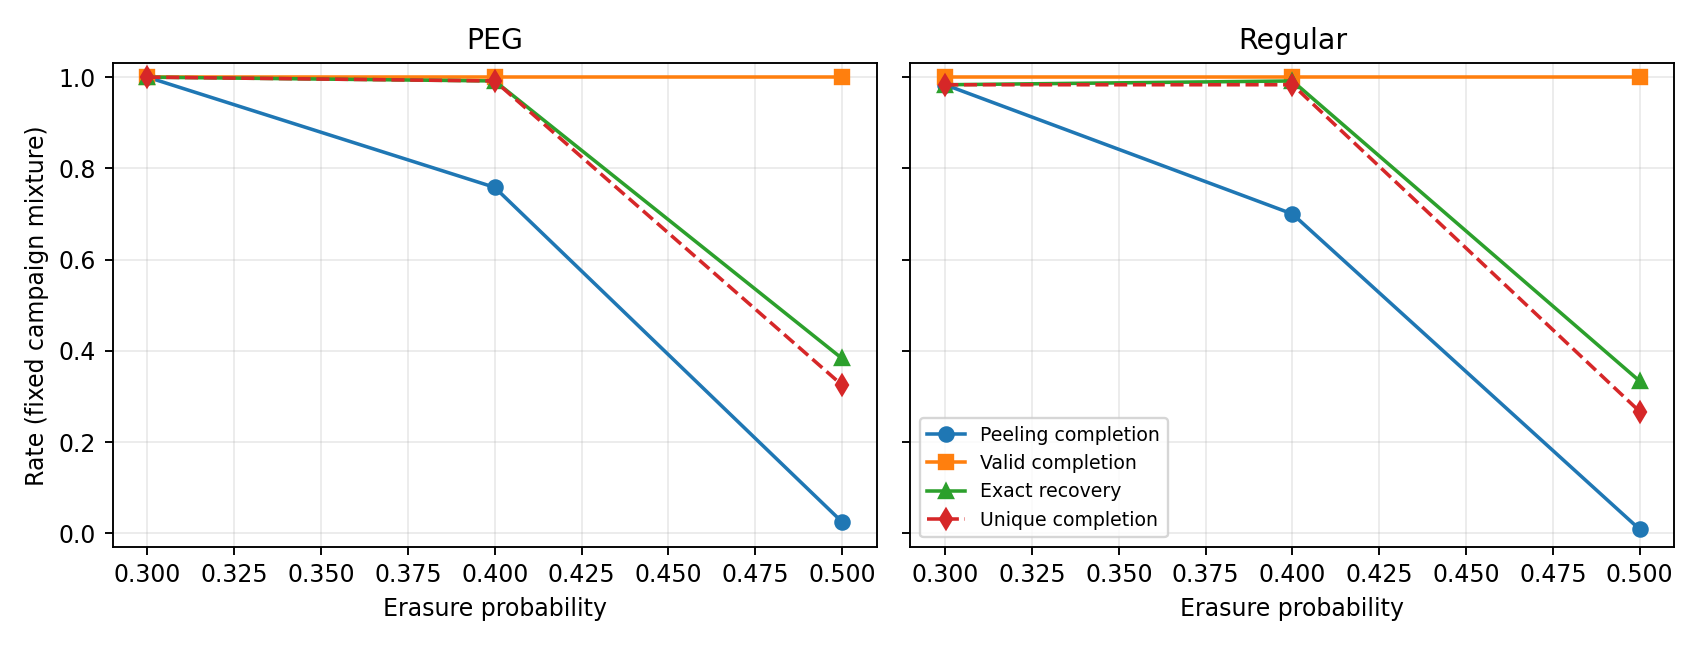
\includegraphics[width=\textwidth]{publication_outputs/fig_completion.png}
\caption{Clean-channel outcomes, displayed separately for each graph
construction. Each point pools 120 trials: four sizes, three matrices
per size and ten observations per matrix at the stated erasure
probability. Valid completion, exact recovery, uniqueness and peeling
completion answer different questions.}
\label{fig:completion}
\end{figure}

\begin{table}
\centering
\small
\setlength{\tabcolsep}{3pt}
\caption{New campaign at erasure probability 0.40: three matrices and ten trials per matrix. C/D is the internal check stage divided by decode time, averaged per trial. The check stage includes comparing checker and producer words.}
\label{tab:new-experiments}
\begin{tabular}{lrrrrrrr}
\toprule
Family & n & Trials & Trace & Residual & Check ms & Direct ms & Mean C/D \\
\midrule
PEG & 128 & 30 & 35.767 & 16.400 & 0.119 & 0.092 & 1.107 \\
PEG & 256 & 30 & 77.367 & 22.233 & 0.241 & 0.186 & 1.147 \\
PEG & 512 & 30 & 190.033 & 11.933 & 0.527 & 0.366 & 1.415 \\
PEG & 1024 & 30 & 389.100 & 22.900 & 1.109 & 0.741 & 1.376 \\
Regular & 128 & 30 & 33.000 & 18.833 & 0.119 & 0.094 & 0.990 \\
Regular & 256 & 30 & 84.500 & 15.900 & 0.247 & 0.184 & 1.243 \\
Regular & 512 & 30 & 174.133 & 32.467 & 0.530 & 0.375 & 1.229 \\
Regular & 1024 & 30 & 377.933 & 33.567 & 1.102 & 0.739 & 1.346 \\
\bottomrule
\end{tabular}
\end{table}

Table~\ref{tab:new-experiments} filters exactly $\varepsilon=0.40$ and
$\delta=0$; no other erasure probabilities enter its averages.
Trace and residual columns are mean numbers of variables. The check-stage column
reports the internal checker stage of the selected certified repetition;
direct checking reports its separately timed median. For these 240
trials, the mean per-trial relative overhead was 1.232, whereas the mean
checker fraction of total time was 0.522. The checker is therefore a
substantial fraction of the measured pipeline, not negligible overhead.
The corresponding ratios of mean times are 0.859 and 0.462; their
difference from the mean ratios reflects variation across trials. The
complete condition CSV also reports the other channel conditions.

\begin{figure}[t]
\centering
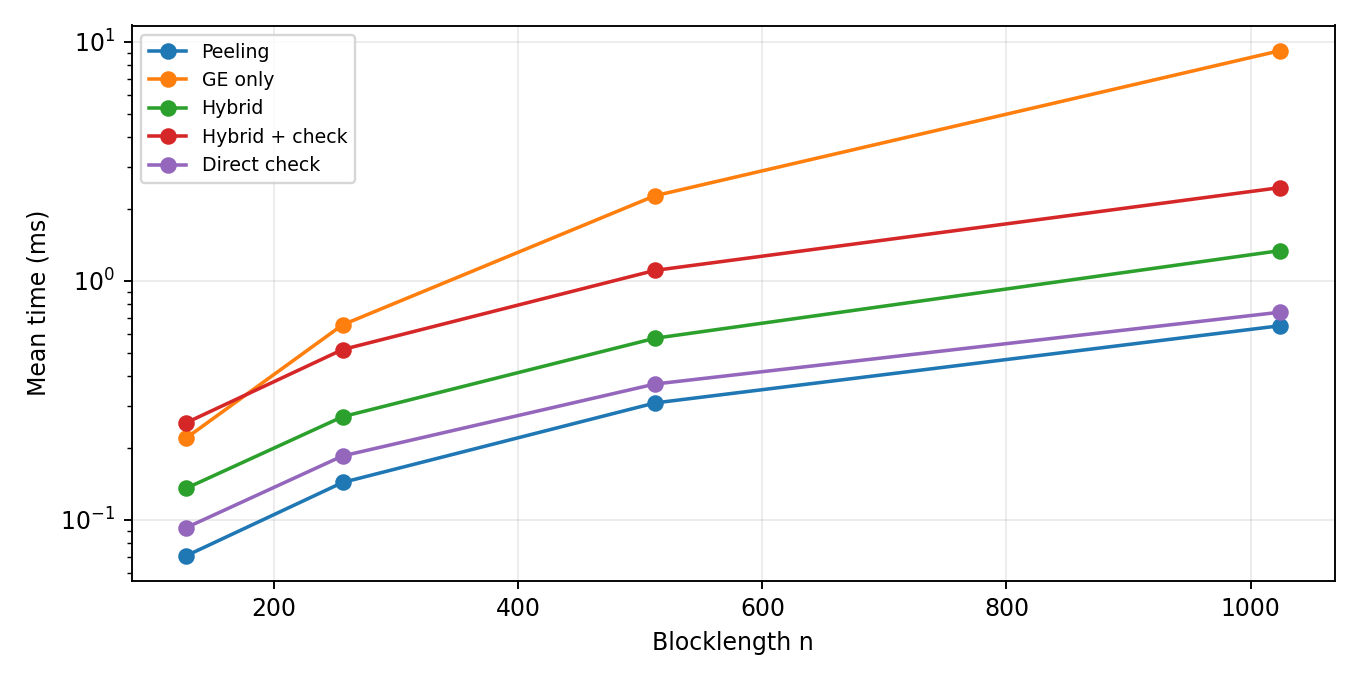
\includegraphics[width=.85\textwidth]{publication_outputs/fig_comparators.png}
\caption{Mean within-trial median times at $\varepsilon=0.40$.
Each size pools 60 observations across both families, with three
matrices per family and ten observations per matrix. Peeling alone may leave
unknowns. Direct checking assumes an already supplied word. Its time
must not be interpreted as a competing decoding latency.}
\label{fig:comparators}
\end{figure}
Figure~\ref{fig:comparators} uses the same algebraic engine across
GE-only and hybrid pipelines. It describes this engine and finite set
of graphs, without attributing a universal speed advantage to the
hybrid strategy or to SELL. Table~\ref{tab:runtime-stages} separates stage means in the same fixed
mixture. Detailed measurements are retained for every observation, so
witness construction and checker cost remain separable from residual
elimination.
\begin{table}
\centering
\small
\setlength{\tabcolsep}{3pt}
\caption{Mean certified runtime stages in milliseconds at erasure probability 0.40, pooled equally over the two named families: six matrices and 60 trials per size. Witness is final vector extraction; row-transform tracking is included in GE. Other includes parsing, output reconstruction and timing overhead; Check includes comparing checker and producer words.}
\label{tab:runtime-stages}
\begin{tabular}{lrrrrrrrr}
\toprule
n & Init & Peel & Residual & GE & Witness & Backsub & Other & Check \\
\midrule
128 & 0.0134 & 0.0137 & 0.0113 & 0.0494 & 0.0001 & 0.0026 & 0.0440 & 0.1187 \\
256 & 0.0266 & 0.0310 & 0.0200 & 0.1019 & 0.0001 & 0.0029 & 0.0872 & 0.2441 \\
512 & 0.0576 & 0.0774 & 0.0380 & 0.2269 & 0.0001 & 0.0035 & 0.1714 & 0.5285 \\
1024 & 0.1229 & 0.1867 & 0.0726 & 0.6213 & 0.0001 & 0.0047 & 0.3375 & 1.1054 \\
\bottomrule
\end{tabular}
\end{table}


\begin{figure}[t]
\centering
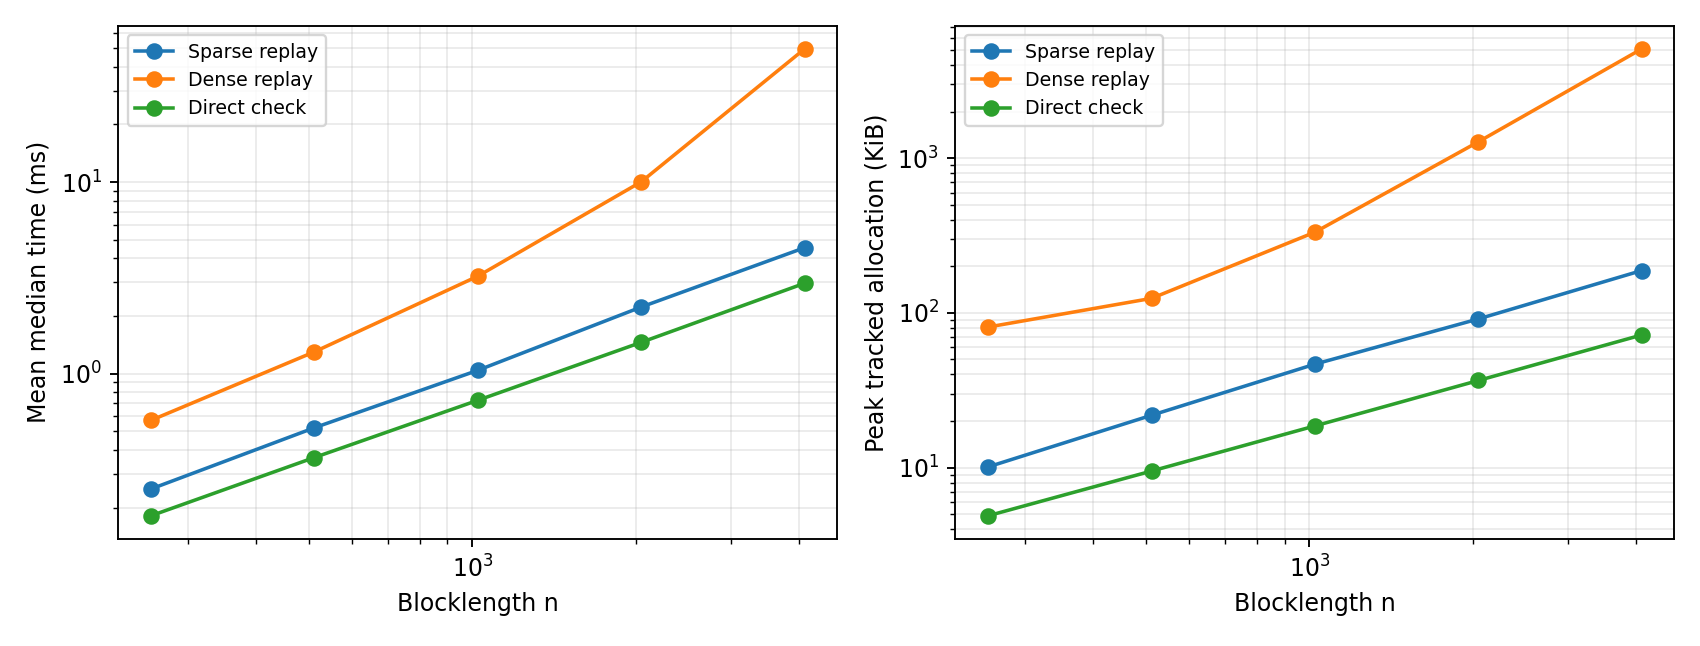
\includegraphics[width=\textwidth]{publication_outputs/fig_checker_scaling.png}
\caption{Independent checker scaling experiment. Time points average
18 within-trial medians (three matrices and six observations); allocation
points average three separately profiled calls, one per matrix. Both
axes of each panel are logarithmic. Allocations exclude preexisting
inputs. The dense and sparse replay implementations check the same
certificates.}
\label{fig:scaling}
\end{figure}
At $n=4096$, mean sparse replay took 4.546\,ms, direct checking
2.966\,ms, and dense replay 49.574\,ms. Corresponding incremental
tracked peaks were approximately 188, 72 and 5094\,KiB.
Thus direct checking was faster and used less additional memory than
trace replay. Both establish the same final parity and visible-coordinate
agreement. Replay additionally checks that each declared assignment is
justified by a degree-one constraint in the preceding operational state.
The measured costs compare complete checker implementations; they do not
isolate the cost of an individual replay step. The fitted time exponents were
1.046 (95\% matrix-bootstrap interval $[1.033,1.062]$) for sparse replay,
1.006 ($[1.003,1.008]$) for direct checking, and
1.583 ($[1.555,1.617]$) for dense replay. The observed sparse exponent
is slightly above one; we do not force a linear fit or treat its
interval as a proof of asymptotic complexity. The abstract sparse bound
in Section~\ref{sec:cost} instead follows from counting incidence
visits in the stated model. Dense scans and Python/runtime effects
prevent identifying every measured implementation with that model.

\begin{figure}[t]
\centering
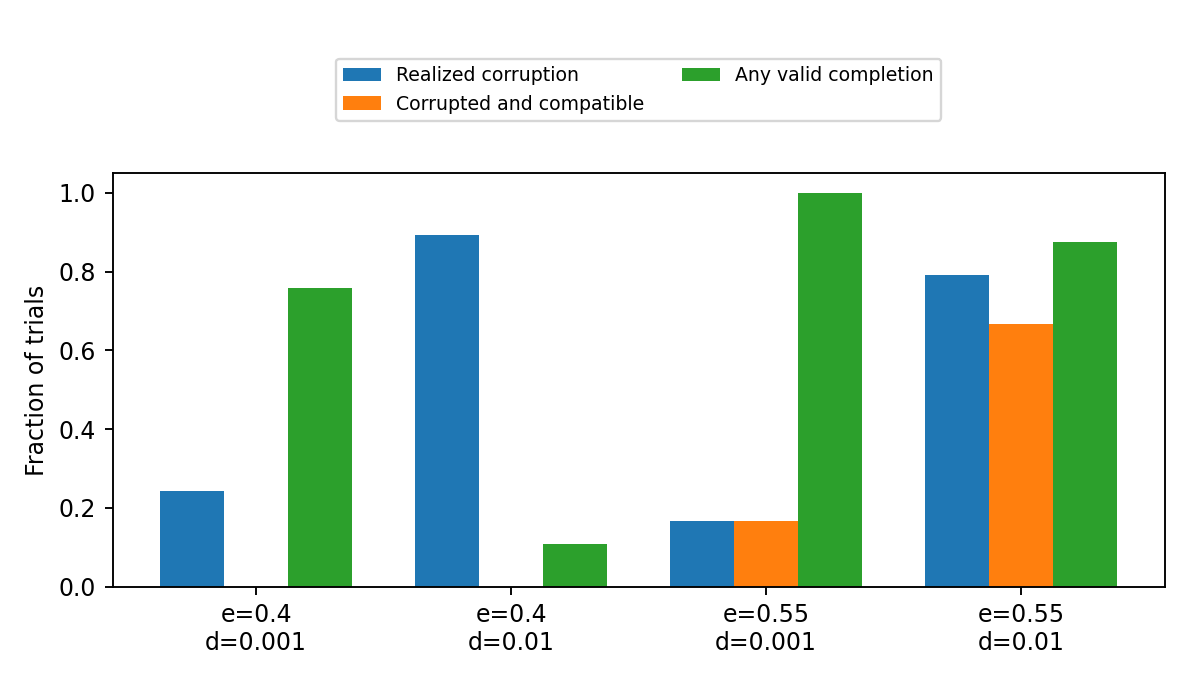
\includegraphics[width=.82\textwidth]{publication_outputs/fig_corruption.png}
\caption{Visible-bit corruption: each group has 120 trials, pooling
two families, two sizes, three matrices and ten observations per
matrix. All bars use that same denominator. ``Corrupted and compatible''
is not conditional on realized corruption; it is a subset of the
``Realized corruption'' bar.}
\label{fig:corruption}
\end{figure}
Of 480 corruption trials, 229 realized no flip. Of the 251 with at
least one flip, 151 were incompatible and yielded accepted failure
certificates; 100 remained compatible and yielded accepted success
certificates. In this fixed campaign, incompatibility exposed
$151/251\approx60.2\%$ of actually corrupted inputs. The remaining
$100/251\approx39.8\%$ cannot be rejected merely for lacking a
completion. Figure~\ref{fig:corruption} uses unconditional trial
fractions, so its bars must not be confused with these conditional
rates. This is algebraic compatibility detection, not a guarantee
against every BEC violation.

\paragraph{Reproducibility and negative evidence.}
The runner checks the complete declared trial grid, preserves all
outcomes, checks matrix fingerprints and records raw-data hashes.
An analysis-stage serialization error and a missing table-rendering
dependency were repaired after all measurements had finished; the
complete original measurements were retained and only analysis was
rerun. Both the executed measurement source and corrected analysis
source are identifiable in the artifact. Tables and figures are
generated from the CSVs by the script and reproducibility notebook.
Finite adversarial tests include malformed domains and certificate
lengths, altered values and indices, invalid orderings, and valid
partial or independently commuting traces. Their observed acceptance
or rejection is test evidence, not a theorem about the Python runtime.
The direct-check advantage, nonunique completions, compatible corruption
and finite-size superlinear fits are retained rather than filtered
from the scientific conclusions.


\section{Related work}\label{sec:related}
The decoding and algebraic foundations are established. Gallager introduced
LDPC codes \cite{Gallager1962}. Iterative erasure correction is developed
in \cite{LubyMitzenmacherShokrollahiSpielman2001}, and finite-length
stopping-set analysis in \cite{DiEtAl2002Stopping}.
Burshtein and Miller combine iterative decoding with algebraic methods
for BEC maximum-likelihood decoding \cite{BurshteinMiller2004ML}.
These results supply the algorithmic setting of the present paper.
Our residual bijection and finite-field alternative articulate the
success/failure certificate contract for that setting rather than
introducing a new hybrid decoder or channel threshold.

Certifying algorithms separate producing a result from checking its
witness \cite{McConnellEtAl2011}. Alkassar and coauthors connect
high-level witness properties with verified checker implementations
\cite{AlkassarEtAl2013}; proof-carrying code supplies a related division
for code-safety evidence \cite{Necula1997PCC}. We apply this producer/checker
organization to a declared local trace and its residual result.
Linear-programming decoding also connects decoding to optimization
guarantees \cite{FeldmanWainwrightKarger2005LP}. Its relaxation-based
optimality setting differs from the BEC feasibility predicate and local
trace explanation checked here.

Linear logic provides the distinction between consumable and reusable
resources \cite{Girard1987}, and focusing structures proof search
\cite{Andreoli1992Focusing}. Nigam and Miller study algorithmic
specifications using subexponential mechanisms richer than the two
persistent zones used here \cite{NigamMiller2009SELL}.
Our operational resource presentation uses this vocabulary to expose
pending work and reusable knowledge. Proposition~\ref{prop:sem-label-erasure}
then identifies the label distinction as inessential to these particular
transitions. This representation result complements
Theorem~\ref{thm:sem-adequacy}; neither is a correspondence theorem for a
SELL sequent calculus or focused proof search.

Formal coding theory supplies a closer algorithmic antecedent as well.
Affeldt, Garrigue and Saikawa formalize linear error-correcting codes in
Coq, including a BEC sum-product decoder with a terminating fixed-point
construction and approximation invariants, and extract an LDPC
sum-product implementation \cite{AffeldtGarrigueSaikawa2020}.
Our emphasis is the exact chronological event trace of delayed
propagation, its logged normal form, and the success/failure witnesses
for the residual system. The canonical Lean development formalizes this
specific correspondence with an explicit boundary to raw multisets and
independent Python code.

Recent work illustrates other certification targets in coding theory.
Ehatamm and coauthors develop Lean-based quantum-code distance
certificates through verified reductions to satisfiability
\cite{EhatammEtAl2026LeanQEC}. Krishnamoorthy and coauthors study
certificates for degenerate quantum-decoding optimality using
partition-function comparisons \cite{KrishnamoorthyEtAl2026CertifiedQ}.
These 2026 preprints concern distance and comparison of quantum error
classes, respectively. Their target properties differ from the BEC
trace/feasibility contract.

Relative to these cited developments, the specific issue addressed here
is the connection between an asynchronously maintained residual state
and an exact, independently checkable operational explanation.
Theorem~\ref{thm:sem-adequacy} supplies that connection for arbitrary
interleavings, and the residual certificate theorems extend it to either
a compatible completion or an infeasibility witness. This is the positive
scope of the contribution assessed against the reviewed literature;
we make no field-wide priority claim for its combination or for the
abstract simulation principle used to organize its proof.

\section{Conclusion and limitations}\label{sec:limitations}
Delayed propagation separates the stored residual resources of an
asynchronous decoder specification from its actual operational state.
The pending-incidence invariant quantifies this separation, and
propagation normalization recovers the unique fully updated context.
The principal result, Theorem~\ref{thm:sem-adequacy}, proves exact
correspondence in both directions: arbitrary rewrite interleavings emit
valid operational traces, and each prescribed valid trace has a realization
with its precise logged normalized endpoint. The abstract proposition
isolates the forward simulation, normalization and local lifting on which
this result depends; empty and partial traces require no maximality
assumption.

The residual bijection connects this trace semantics to a complete
success/failure contract. A residual solution supplies a compatible
codeword; a left-kernel separator excludes every compatible word.
The Lean development proves the canonical LDPC correspondence and the
stated certificate results, while finite tests and experiments assess
an independent executable implementation. The representation table in
Section~\ref{sec:lean} marks the mathematical, mechanized and tested
connections separately.

The SELL-style presentation exposes reusable knowledge and consumable
pending work. Proposition~\ref{prop:sem-label-erasure} shows that its two
persistent labels can be merged for these rules, thereby separating a
useful specification discipline from what the operational proof needs.
No SELLF adequacy or expressiveness separation follows.

Trace replay certifies a declared local operational explanation, not the
producer's true internal history. Direct checking establishes the same
final-word validity condition and was faster in the retained measurements.
A compatible completion need not be unique or equal the transmitted word;
visible corruption can remain algebraically compatible. The supplied
matrix, observation, checker and execution environment remain within the
stated trust boundary. Python is not extracted from Lean, and the abstract
proposition and raw-representation bridge are manuscript proofs.

The experiments concern the recorded graph constructions, finite sizes
and host. Three matrices per condition limit ensemble inference, and
fitted scaling exponents are descriptive, not asymptotic guarantees.
The additional trace evidence has measured checking costs; it supports
neither a universal speed advantage nor universal corruption detection.

\AtBeginEnvironment{thebibliography}{\interlinepenalty=10000}
\bibliographystyle{alphaurl}
\bibliography{SELLTCFULL}
\end{document}
